\begin{center}
  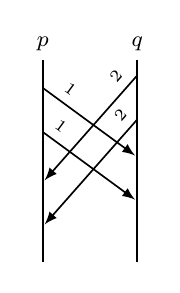
\begin{tikzpicture}[>=stealth,node distance=3.4cm,shorten >=1pt,
  every state/.style={text=black, scale =0.7}, semithick,
    font={\fontsize{8pt}{12}\selectfont}]

\begin{scope}[shift = {(8,0.75)}, scale = 0.8]
%	\draw (0.75, -4) node{\textbf{(b)}};
  %MACHINES
  \draw (0,0) node{$p$} ;
  \draw (1.5,0) node{$q$} ;
  \draw (0,-0.25) -- (0,-3.5) ;
  \draw (1.5,-0.25) -- (1.5,-3.5);
  %MESSAGES

  \draw[>=latex,->] (0, -0.7) -- (1.5, -1.8) node[pos=0.2, sloped, above] {$\amessage_1$};
  \draw[>=latex,->] (0, -1.4) -- (1.5, -2.5) node[pos=0.1, sloped, above] {$\amessage_1$}; %{$\amessage_1'$};
  %\draw[>=latex,->, dashed] (0, -2.5) -- (1.25, -3.25) node[pos=0.55, sloped, above] {$\amessage_1''$};

  \draw[>=latex,->] (1.5, -0.5) -- (0, -2.2) node[pos=0.1, sloped, above] {$\amessage_2$};
  \draw[>=latex,->] (1.5, -1.2) -- (0, -2.9) node[pos=0.05, sloped, above] {$\amessage_2$};
  % \node[rotate = 90, left]at (1.13, -0.65) {$\cdots$};
  % \node[rotate = -90, right]at (0.1, -0.65) {$\cdots$};

\end{scope}

\end{tikzpicture}
\captionof{figure}{MSC $\mscWS$}
\label{fig:msc_W_S}
\end{center}
